
\section{Komplexe Zahlen}

\begin{minipage}[c]{0.5\textwidth}
	\centering
	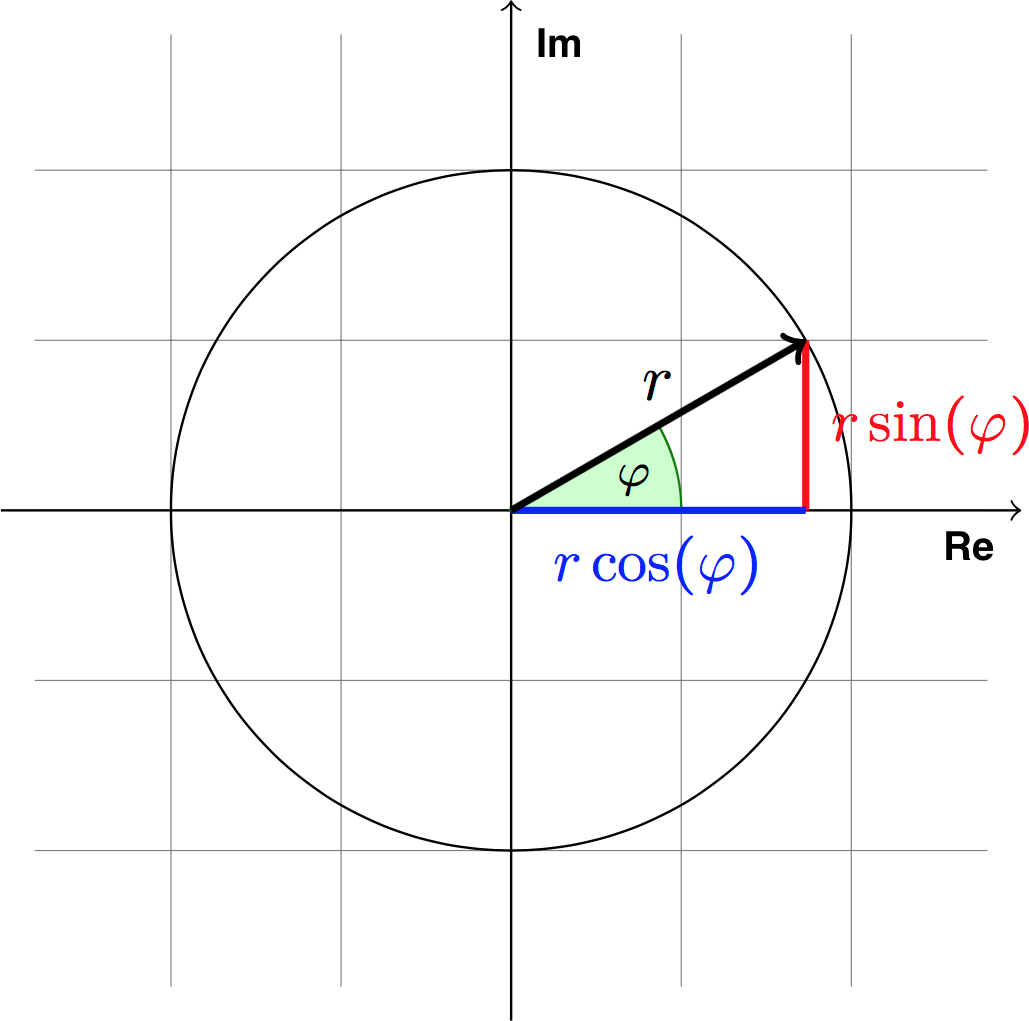
\includegraphics[width=\linewidth,keepaspectratio=true]{images/polarform}
\end{minipage}
%
\begin{minipage}[c]{0.5\textwidth}
	\begin{equation*}
	\begin{split}
	z & = x + iy = r(\cos(\varphi) + i\sin(\varphi)) = re^{i\varphi} \\
	r & = |z| = \sqrt{x^2 + y^2} \\
	\arg(z) & = \varphi  = \arctan(\frac{y}{x}) \quad \text{(je nach Quadrant)}  \\
	x & = r\cos(\varphi) \\
	y & = r\sin(\varphi) \\
	zw & = (re^{i\varphi})\cdot(se^{i\psi}) = rse^{i(\varphi + \psi)} \\
	\sqrt[q]{z} & = \sqrt[q]{s}e^{i\phi}\text{, wobei }\phi = \frac{\varphi}{q} \mod \frac{2\pi}{q} \\
	e^{i(\frac{\pi}{2} + 2\pi k)} & = i,\ e^{i\pi} = 1, \ e^{-i\pi} = -1
	\end{split}
	\end{equation*}
\end{minipage}

\begin{minipage}[c]{0.5\textwidth}
	\begin{equation*}
	\begin{split}
	(a,b) \cdot (c, d) & = (ac-bd, ad+bc) \\
	\overline{z} & = x - iy\\
	z^{-1} & = \frac{\overline{z}}{|z|^2} \\
	i & = \sqrt{-1}\\
	\end{split}
	\end{equation*}
\end{minipage}
%
\begin{minipage}[c]{0.5\textwidth}
	\begin{equation*}
	\begin{split}
	i^2 & = -1 \\
	|z|^2 & = z\overline{z} \\
	|zw|^2 & = (zw) \cdot \overline{(zw)} = |z|^2|w|^2
	\end{split}
	\end{equation*}
\end{minipage}
\figurename
